\documentclass{article}[18pt]
\usepackage{../../../../format}
\lhead{Networks and Systems - Distributed Systems}


\begin{document}
\begin{center}
\underline{\huge From middleware to web services}
\end{center}
\section{Middleware for system integration}
RPC, Java RMI and Python PYRO
\begin{itemize}
	\item Closely follow the traditional program development process that creased an application based on 
	\begin{enumerate}
		\item Program libraries integration
		\item Parameter passing
	\end{enumerate}
	\item Do not require developers to deal with socket programming when implementing programs that support remote communication
	\item Have a performance issue due to synchronous communication
\end{itemize}
COBRA
\begin{itemize}
	\item Still follow the programming library approach
	\item Similar to Java RMI: provide object request broker (ORB) define the interface definition language (IDL)
	\item Integrate components developer by different programming languages
\end{itemize}
\section{Message-Oriented Middleware (MOM)}
\begin{itemize}
	\item We need something more loosely coupled
	\item Communication using messages
	\item Messages stored in message queues
	\item Message servers decouple client and server
	\item Various assumptions about message content
	
\end{itemize}

\begin{center}
	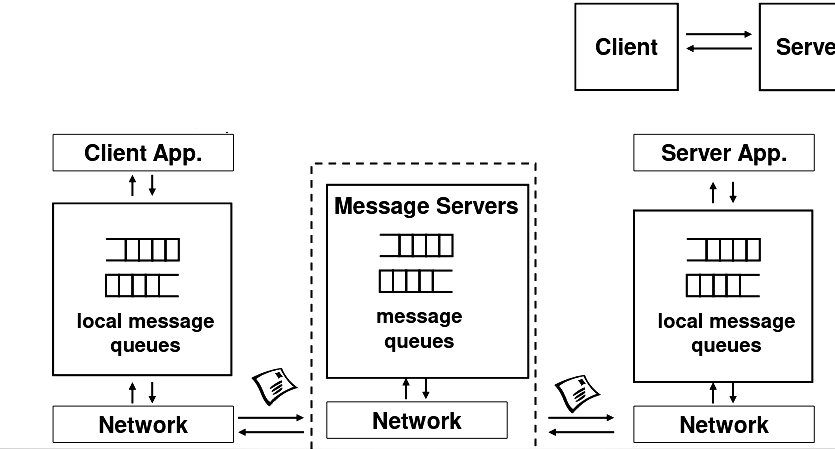
\includegraphics[scale=0.7]{MOM}
\end{center}
\subsection{Properties of MOM}
Asynchronous interaction
\begin{itemize}
	\item Client and server are only loosely coupled
	\item Messages are queued
	\item Good for application integration
\end{itemize}
Support for reliable delivery service
\begin{itemize}
	\item Keep queues in persistent storage
\end{itemize}
Processing of messages by intermediate message server(s)
\begin{itemize}
	\item May do filtering, transforming, logging
	\item Networks of message servers
\end{itemize}
Natural for database integration
\section{Java Message Service (JMS)}
\begin{itemize}
	\item API specification to access MOM implementations
	\item Two modes of operations 
	\item Point to point
	\begin{itemize}
		\item One to one communication
	\end{itemize}
	\item Publish/subscribe
	\begin{itemize}
		\item One to many communication
	\end{itemize}
	\item JMS server implements JMS API 
	\item JMS clients connect to JMS servers
	\item Java objects can be serialised to JMS messages
\end{itemize}
\section{Web services}
Use well known web standards for distributed computing\\
Communication
\begin{itemize}
	\item Message content expressed in XML
	\item Simple Object Access Protocol (SOAP) - lightweight protocol for sync/async communication
\end{itemize}
Service description
\begin{itemize}
	\item Web Services Description Language (WSDL) - interface description for web services
\end{itemize}
Service Discovery
\begin{itemize}
	\item Universal Description Discovery and Integration (UDDI) - directory with web service description in WSDL
\end{itemize}

\begin{center}
	\includegraphics[scale=0.5]{"Web Services"}
\end{center}
\subsection{Attributed of Web-Services}
Web based protocols - Web services based on HTTP are designed to work over the public internet. The use of HTTP for transport means these protocols can traverse firewalls,l and can work in a heterogeneous environment\\
\\
Interoperability - SOAP defines a common standard that allows differing systems to interoperate\\
\\
XML based - The Extensible Markup Language is a standard framework for creating machine readable documents
\section{REST and JSON}
REST
\begin{itemize}
	\item An architectural style, treating the web as a resource centric application 
	\item Each URL in a RESTful application represents a resource
\end{itemize}
JSON
\begin{itemize}
	\item An open standard format that uses human readable text to transmit data objects consisting of attribute-value pairs
	\item Provide lightweight communication
\end{itemize}




\end{document}